\documentclass[a4paper,french]{paper}
\usepackage{../../_latex_assets/villemejane_iogs_ceti}

%Informations about this document 
%------------------------------------------
\def\module{Conception Electronique pour le Traitement de l'Information}
\def\moduleAbrege{5N-027-SCI / CéTI}
\def\annee{}

\def\titre{Bloc 3 / Transmission par la lumière}
\author{Julien VILLEMEJANE}

\subtitle{Bloc3}
\institution{LEnsE / Institut d'Optique Graduate School}

\title{\titre}
\begin{document} 
%Beginning First Page. 
%------------------------------------------
\enteteThematiqueObligatoire{}

%Beginning Content. 
%------------------------------------------
\vspace{-1cm}
%%%%%%%%%%%%%%%%%%%
\encadreTDExo{1 - Emettre une information lumineuse}{
En se basant sur une \textbf{LED IR} de type SFH415.

Proposer un montage émetteur permettant d'obtenir un flux lumineux sinusoïdal sans risque pour la LED, et donner les paramètres des différentes sources utilisées et des autres éléments du montage.
}

%%%%%%%%%%%%%%%%%%%
\encadreTDExo{2 - Transmettre une information par la lumière}{
En se basant sur une \textbf{LED IR} de type SFH415 et une \textbf{photodiode} de type SFH229, on souhaite réaliser un système de transmission d'information par la lumière.

On se propose dans un premier temps d'utiliser le montage "simple" de photodétection.

\begin{center}
	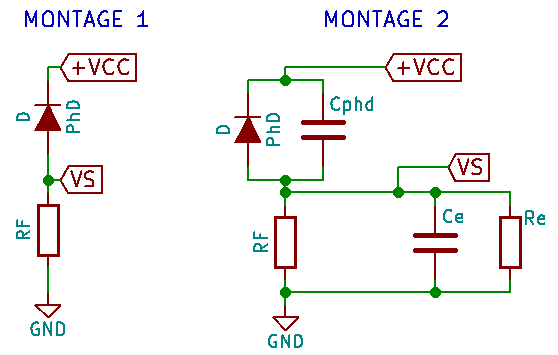
\includegraphics[width=7cm]{images/photodetection_simple_modele.png}
\end{center}

A quoi correspondent les deux montages proposés ?

Donner la fonction de transfert du montage en fonction du flux lumineux reçu.

Quelle est alors la limite en fréquence d'un tel montage ? Peut-on transmettre des données binaires ?
} 

%%%%%%%%%%%%%%%%%%%
\encadreTDExo{3 - Transmettre une information par la lumière - transimpédance}{
En se basant sur une \textbf{LED IR} de type SFH415 et une \textbf{photodiode} de type SFH229, on souhaite réaliser un système de transmission d'information par la lumière.

On se propose dans un premier temps d'utiliser le montage de photodétection de type transimpédance.

\begin{center}
	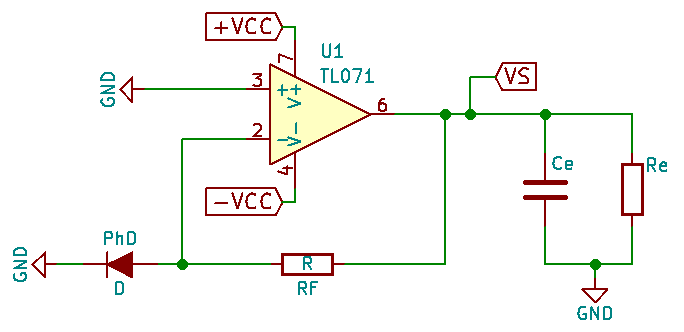
\includegraphics[width=8cm]{images/photodetection_transimpedance.png}
\end{center}

Donner la fonction de transfert du montage en fonction du flux lumineux reçu.

Quelle est alors la limite en fréquence d'un tel montage ? Peut-on transmettre des données binaires ?
}


%%%%%%%%%%%%%%%%%%%
\encadreTDExo{4 - Modéliser le montage transimpédance}{
Dans l'exemple précédent, nous avons supposé l'amplificateur linéaire idéal. 

On prendra le modèle suivant pour l'amplificateur linéaire :

$$V_S = \frac{A_0}{1 + j \cdot \frac{\omega}{\omega_0}} \cdot (V^+ - V^-)$$

Calculer la fonction de transfert $T(j\cdot \omega) = V_S /  i_{PHD}$ du montage suivant :
} 


\begin{figure}[!h]
\centering
\begin{circuitikz} 
	\node [op amp](A1) at (0,0){\texttt{ALI1}};
	\draw (A1.-) to[short] ++(-.5,0) coordinate(A) to[short] ++(0,1.5) coordinate(B) to[R=$R_F$, i=$i_R$] (B -| A1.out) to[short, -*] (A1.out);
	\draw (A1.- -| -5,0) node[ground]{};
	\draw (A1.- -| -5,0) to[I, invert, i=$i_{Phd}$, *-*] (A);
	\draw (A1.- -| -5,0) -- ++(0,1.5) to[C, l=$C_{Phd}$, i=$i_C$, -*] (B);
	\draw (A1.+) to[short] ++(0,-0.5) node[ground]{};
	\draw (A1.out) -- ++(1,0) coordinate(D);
	\draw (2.2,-2.1) edge[->, color={red}] (2.2,-0.3);
	\node[text={red}] (Vs) at (1.7,-1.2){$V_s$}; 
	\draw (D) -- ++(1,0) to[C,l=$C_{e}$, *-*] ++(0,-2.5) coordinate(G);
	\draw (G) node[ground]{};
	\draw (G) -- ++(2,0) to[R,l=$R_e$] ++(0,2.5) -- ++(-2,0);
\end{circuitikz}
\end{figure}


%%%%%%%%%%%%%%%%%%%
\encadreTDExo{5 - Détecter un obstacle}{
	On souhaite détecter un obstacle à une certaines distances. Proposer une solution basée sur une LED IR et un photodétecteur.
}

%%%%%%%%%%%%%%%%%%%
\encadreTDExo{6 - Transporter plusieurs informations par la lumière}{
	On souhaite rendre plus spécifique une communication par la lumière, et pourquoi pas transporter plusieurs informations différentes sur un même canal lumineux.
	
	Proposer une solution.
}

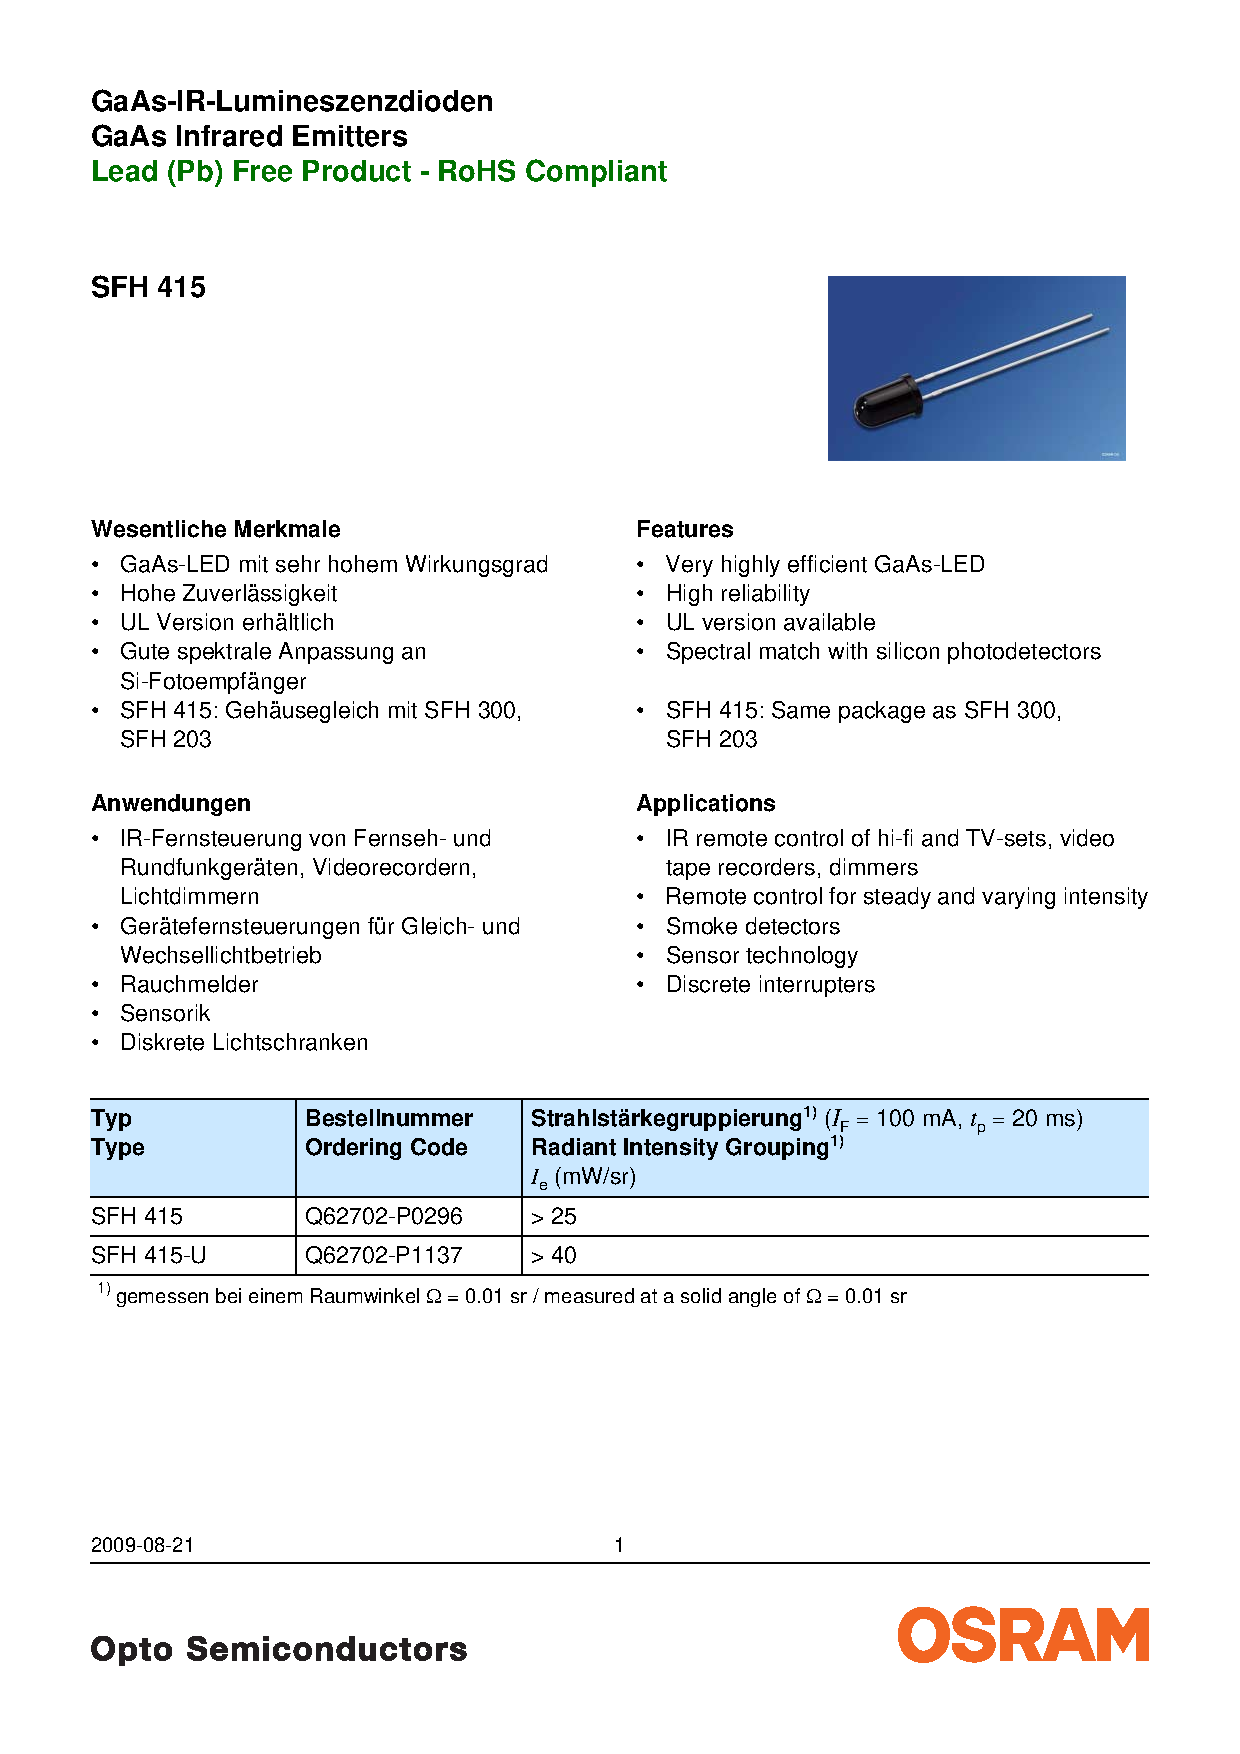
\includepdf[pages=1-3]{doc/SFH415.pdf}

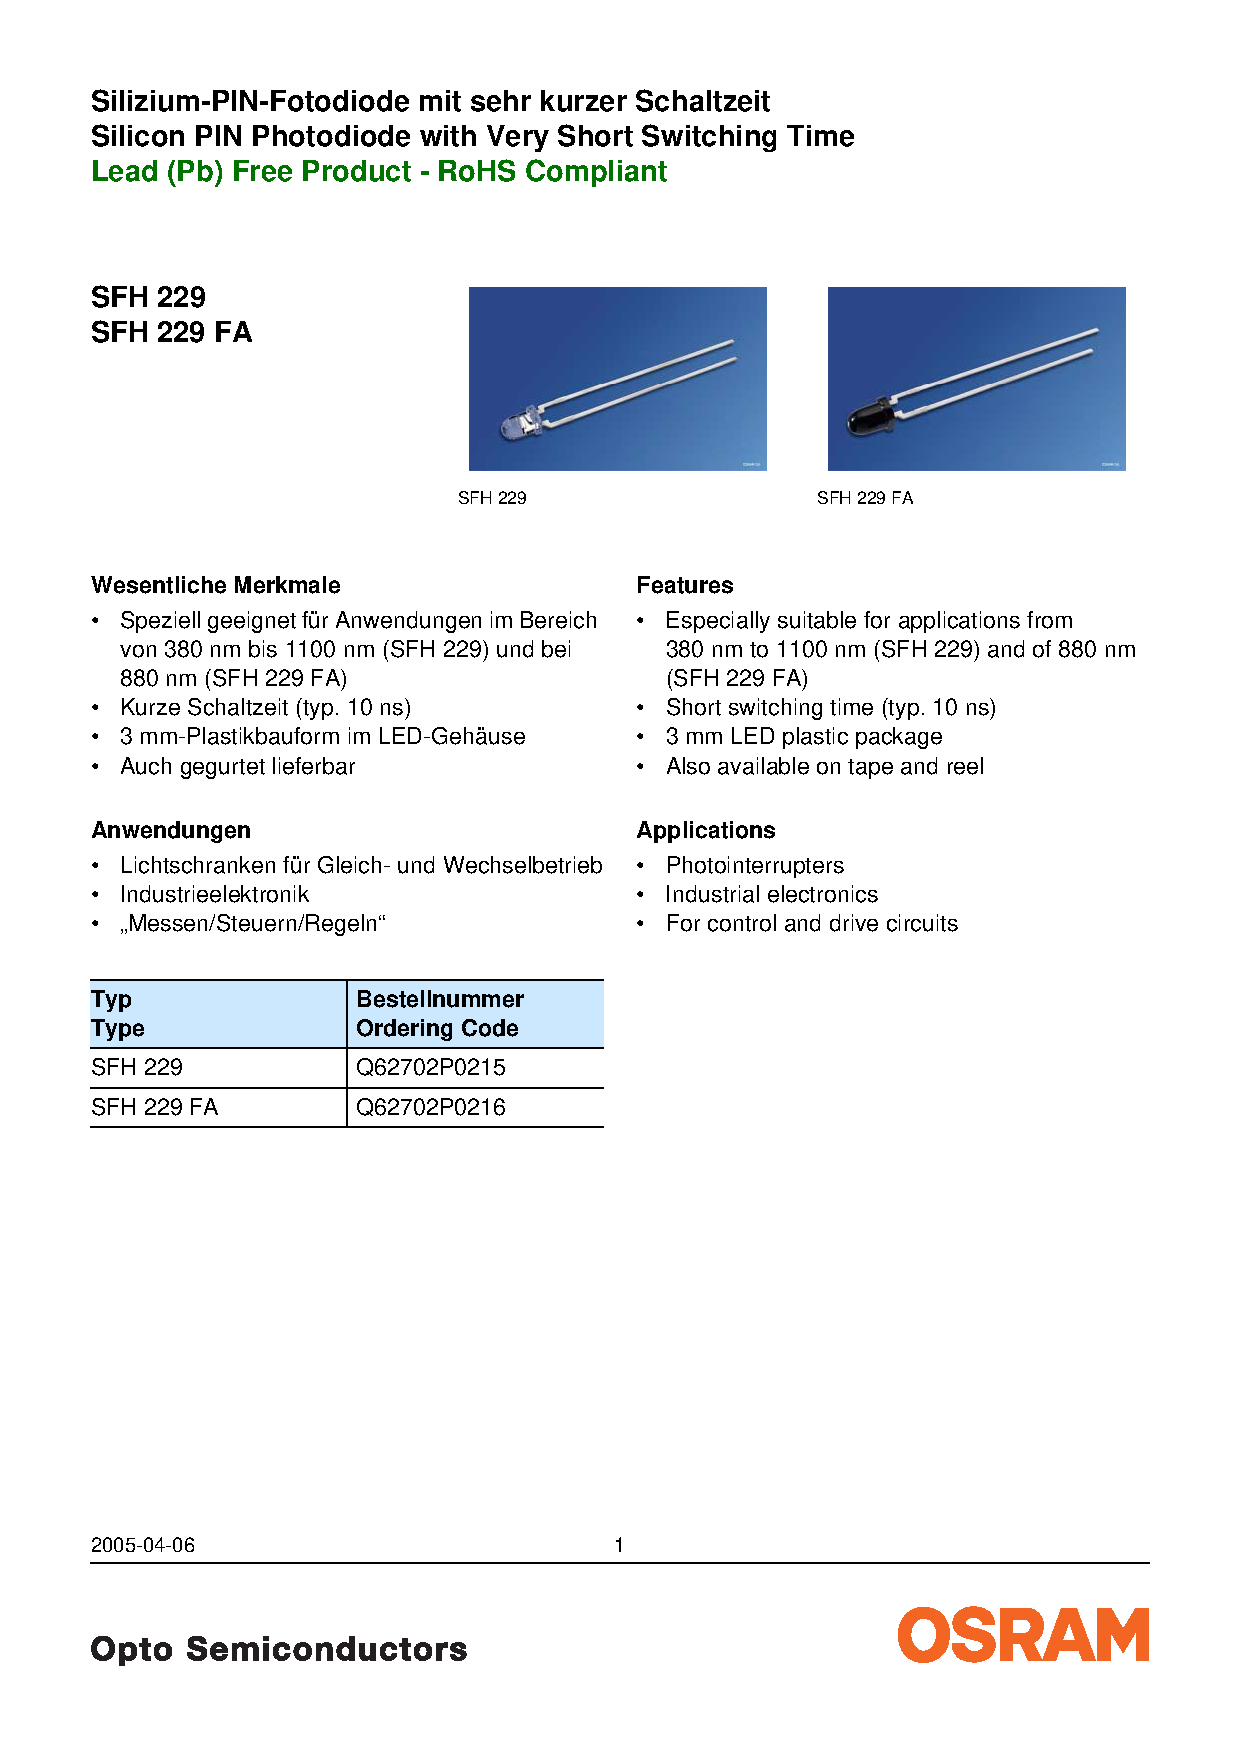
\includepdf[pages=1-5]{doc/SFH229.pdf}

\end {document}